\subsection{Platonische Körper}
In den vorherigen Kapiteln haben wir uns mit der Klassifizierung der endlichen Untergruppen der orthogonalen Gruppen im Zweidimensionalen beschäftigt. Dabei haben wir feststellen können, dass es für die Klassifizierung ausreicht nur Gruppen zu betrachten, die zu regulären Polygonen gehören, wie zum Beispiel die Gruppe $\mathcal{C}_4$, die zu einem Quadrat gehört. Da wir uns nun damit beschäftigen wollen, wie wir die endlichen Untergruppen der orthogonalen Gruppe im Dreidimensionalen klassifizieren können, liegt es nahe sich mit regulären Polyedern zu befassen.\\
Wir beginnen mit einigen Definitionen: 
\begin{defi}[Einfaches Polyeder]
	Ein Polyeder heißt einfach, wenn seine Oberfläche sich stetig in eine Kugelfläche überführen lässt, das heißt einfach Polyeder haben keine \enquote{Löcher}. \citep[211]{Mainzer1988}
\end{defi}
\textbf{Beispiele für ein einfaches und ein nicht-einfaches Polyeder}
\begin{defi}[Konvexes Polyeder]
	Ein Polyeder heißt konvex, wenn zu je zwei Punkten aus dem Inneren des Polyeders auch deren Verbindungsstrecke ganz im Polyeder liegt. \citep[51]{Mueller2012}
\end{defi}
\begin{defi}[Reguläres Polyeder]
	Ein konvexes Polyeder heißt regulär, wenn alle Flächen zueinander kongruente regelmäßige Vielecke sind und in jeder Ecke gleich viele Vielecke zusammenstoßen. \citep[51]{Mueller2012}
\end{defi}
Diese Definitionen werden uns erneut im Beweis des Eulerschen Polyedersatzes begegnen. Es gibt genau fünf reguläre Polyeder.\\
\begin{figure}[H]
    \centering
    
\includegraphics[width=0.9\linewidth]{grafiken/platonische_koerper.pdf}
    \caption{Die fünf regulären Polyeder - Tetraeder, Würfel, Oktaeder, Dodekaeder und Ikosaeder.}
    \label{fig:grafiken/platonische_koerper}
\end{figure}
Für diesen Sachverhalt wurden verschiedene Beweise formuliert, von denen wir zwei nachvollziehen bzw. gegenüberstellen wollen. \\
Wir werfen nun zunächst einen Blick zurück in die Geschichte und befassen uns mit der Entdeckung der fünf regulären Polyeder und ihrer Bedeutung im Laufe der Jahrhunderte. \\
Bereits im antiken Griechenland wurde erkannt und bewiesen, dass nur fünf platonische Körper konstruiert werden können: Tetraeder, Hexaeder (Würfel), Oktaeder, Ikosaeder und Dodekaeder. Ihr Namensgeber Platon beschrieb die regulären Polyeder etwa 350 v. Chr. im Kontext des naturphilosophischen, kosmologischen Werks "Timaios". Platon war nicht nur von der Vollkommenheit und Symmetrie beeindruckt, sondern insbesondere davon überzeugt, dass vier der platonischen Körper die Strukturen der Elemente Feuer, Wasser, Erde und Luft beschreiben, aus denen der Kosmos besteht. Der Dodekaeder repräsentierte hingegen die göttlich gegebene Konstellation der Himmelskörper.\\
Die erste Niederschrift der Konstruktion mit Lineal und Zirkel findet sich in Euklids mehrbändigen Werk Elemente (Buch XII), das um 300 v.Chr. entstand. Von ihm stammt auch die folgende Begründung, weshalb es nicht mehr als die bekannten fünf platonischen Körper geben kann:
\begin{proof}
a) Zunächst wollen wir überlegen, warum reguläre Polyeder nur aus gleichseitigen Dreiecken, Quadraten oder regelmäßigen Pentagonen bestehen kann. Um überhaupt eine Polyederecke herausbilden zu können, werden mindestens drei Polygone benötigt. \\
Weiter können wir festhalten, dass die Winkelsumme der Kanten, die in der Polyederecke aufeinander treffen, kleiner als der Vollwinkel sein muss, um eine konvexe Ecke zu formen. Anderenfalls, würde die Winkelsumme genau $360^\circ$ betragen, würden die Flächen eine Parkettierung der Ebene bilden. Auch bei mehr als $360^\circ$ wäre hingegen keine Ecke möglich.\\
Die Winkelsumme in regulären n-Ecken kann durch die Formel $(n-2)\cdot 180^\circ$ beschrieben werden (Begründung: Durch das Einzeichnen eines Punktes innerhalb des Polygons kann dieses in Dreiecke unterteilt werden. Die Hinzunahme einer weiteren Ecke erlaubt es uns, genau ein weiteres Dreieck einzuzeichnen. So kann die Zunahme der Winkelsumme um $180^\circ$ mit jeder zusätzlichen Ecke erklärt werden.). Wir erhalten für Dreiecke, Quadrate und regelmäßige Pentagone eine Innenwinkelsumme von $180^\circ, 360^\circ$ bzw. $540^\circ$. Die Winkel in den Ecken sind dementsprechend beim Dreieck $60^\circ$, beim Quadrat $90^\circ$ und im regelmäßigen Fünfeck $105^\circ$ groß. \\
Das regelmäßige Hexagon hat eine Innenwinkelsumme von $720^\circ$, die Winkel in den Ecken messen dementsprechend je $120^\circ$. Drei Hexagone bilden also wegen $3\cdot 120^\circ=360^\circ$ keine konvexe Ecke mehr, natürlich bilden auch vier, fünf, etc. Hexagone keine konvexe Ecke. Auf gleiche Weise sehen wir, dass auch das Aneinanderlegen von drei oder mehr Polygonen mit mehr als sechs Ecken keine konvexe Ecke ergibt.\\
Wir halten fest, dass die Flächen der platonischen Körper nur regelmäßige Polygone mit drei, vier oder fünf Ecken sein können.\\

b) Jetzt wollen wir überlegen wie viele Dreiecke, Quadrate oder Pentagone an jeweils einer Ecke des Polyeders zusammentreffen können. Wir orientieren uns dabei an obiger Argumentation.\\
Gleichseitige Dreieck besitzen Innenwinkel von $60^\circ$. Wir können bis zu fünf dieser Dreiecke an ihren Ecke zu einer konvexen Polyederecke zusammenfügen. Die auf diese Weise entstehenden Körperecken die durch das Aufeinandertreffen von drei, vier oder fünf Dreiecken entstehen sind  $180^\circ, 240^\circ$ bzw. $300^\circ$ groß.\\
Quadrate besitzen Innenwinkel von $90^\circ$. Um den Vollwinkel nicht zu überschreiten bzw. zu erreichen, können wir nur die Mindestanzahl von drei Flächen aneinanderlegen $(3\cdot90^\circ=270^\circ)$.\\
Gleiches gilt, wenn wir regelmäßige Pentagone als Seitenflächen wählen: Nur drei Fünfecke bilden eine konvexe Ecke, die einen Winkel von $324^\circ$ einschließt.\\
Insgesamt erhalten wir drei Polyeder mit dreieckigen Seitenflächen und jeweils einen mit vier- bzw. fünfeckigen Seitenflächen. Genau genommen wissen wir nun erst, dass es nicht mehr als fünf platonische Körper geben kann. Die Existenz haben wir nicht explizit nachgewiesen, jedoch kennen wir die platonischen Körper Tetraeder, Oktaeder und  Ikosaeder (dreieckige Flächen), Hexaeder (viereckige Flächen) und Dodekaeder (fünfeckige Flächen) und damit ist ihre Existenz schließlich auch gesichert. 
\end{proof}
Einige Jahrhunderte später fanden die platonische Körper auch in anderen Disziplinen einen Platz: 
Der Astronom Johannes Kepler konstruierte Ende des 16. Jahrhunderts (1596 in Mysterium Cosmographicum) ineinander verschachtelte Modelle der platonische Körper, um die Umlaufbahnen der bis dato sechs bekannten Planeten (noch unbekannt: Uranus und Neptun) um die Sonne zu beschreiben. Kepler nutzte die Eigenschaft, dass jeder reguläre Polyeder eine Inkugel und eine Umkugel hat. Auf der Inkugel liegen die Mittelpunkte der Seitenflächen des Polyeders, während alle konvexen Ecken auf der Umkugel liegen. Auf diesen Kugelschalen beschreiben die Planeten nach Kepler Kreisbahnen. Die platonischen Körper passte der Astronom so von innen nach außen zwischen den Kugelhüllen ein, dass eine Kugel die Inkugel des Polyeders ist, während die nächste seine Umkugel ist. Dadurch ergab sich folgende Anordnung: Das Oktaeder lag zwischen Merkur und Venus, das Ikosaeder zwischen Venus und Erde, das Dodekaeder zwischen Erde und Mars, das Tetraeder zwischen Mars und Jupiter und das Hexaeder zwischen Jupiter und Saturn.\footnote{http://www.mathe.tu-freiberg.de/~hebisch/cafe/platonische.html}  Wenngleich Keplers Theorie später widerlegt wurde, war er einer der ersten Naturwissenschaftler, der auf geometrische Sachverhalte zur Erklärung astronomischer Phänomene zurückgriff.\\
Leonhard Euler formulierte im 18. Jahrhundert den Eulerschen Polyedersatz, der eine Aussage über das Verhältnis der Anzahlen an Seitenflächen, Kanten und Ecken macht. Wirklich neu ist das Resultat nicht: Vermutlich wussten auch Descartes im 17. Jahrhundert und der Grieche Archimedes bereits von dem Zusammenhang. Insbesondere brauchen wir den \textit{Eulerschen Polyedersatz}, um den angekündigten zweiten Beweis zur Existenz der fünf platonischen Körper führen zu können.\\
Verschiedene Vorstellungen von der Konstruktion der Polyeder legen andere Beweisideen zum Eulerschen Poyledersatz nahe, argumentiert Berendonk in seinem Buch "'Erkundungen zum Eulerschen Polyedersatz". \citep[vgl.][39]{Berendonk2014} Der hier geführte Beweis nach von Staudt folgt der Vorstellung, dass Polyeder aus Netzen entstehen.\footnote{Die Beweise von Euler selbst und Cauchy, die Berendonk ebenfalls ausführt und erläutert, sind hingegen am plausibelsten, wenn Polyeder als Festkörper bzw. als aus einzelnen Polygonen zusammengesetzt gedacht werden.}\\
Von Staudt greift in seinem Beweis auf grundlegende Begriffe der Graphentheorie zurück, die wir vorab einführen wollen. Die Graphentheorie als Teilgebiet der Topologie befasst sich mit der Art und Weise, wie Figuren verbunden sind. Die von uns betrachteten Polyeder haben die zentrale Eigenschaft, dass ihre Seitenflächen eine einzige, grenzenlose Oberfläche bilden. Die Kanten sind in diesem Sinne Kurven auf dieser Oberfläche, von denen drei oder mehr dort aufeinander treffen, wo sich die Ecken des Polyeders befinden. 
\begin{bem} 
Die $\mathcal{N}_0$ Ecken und $\mathcal{N}_1$ Kanten eines $\mathcal{N}_2$-flächigen regelmäßigen, konvexen Polyeders ergeben einen speziellen \textit{Graphen}, der eine Menge aus $\mathcal{N}_0$ Punkten bzw. \textit{Knoten} und $\mathcal{N}_1$ Segmenten bzw. \textit{Zweigen} ist. Damit ein Graph \textit{zusammenhängend} ist, muss die Ungleichung $N_{1} \geq N_{0}-1$ erfüllt sein. 
Einen zusammenhängenden Graphen, der außerdem keine \textit{Zykel} (z.B. durch Polygone) aufweist, nennen wir einen \textit{Baum}. Für Bäume gilt sogar die Gleichung $N_{1} = N_{0}-1$. 
\end{bem}
Coxeter fasst die Erkenntnisse wie folgt zusammen: mit anderen Worten ist das Polyeder mit $\mathcal{N}_0$ Ecken, $\mathcal{N}_1$ Kanten und $\mathcal{N}_2$ Flächen ein regulärer Graph, d.h. die $\mathcal{N}_1$ Kanten und $\mathcal{N}_0$ Ecken schaffen eine Partition der unbegrenzten Oberfläche bestehend aus $\mathcal{N}_2$ polygonalen Gebieten (Coxeter,6).\\
Aus einem gegebenen Graphen können wir einen zweiten ableiten, der auf derselben Oberfläche liegt -den so genannten \textit{dualen Graphen}. 
%\begin{defi}
%Der duale Graph zu einem planaren Graph G ist ein Graph, der zu jeder Fläche von G einen Knoten hat. Außerdem gibt es für jede Kante in G eine Kante im dualen Graph, die in zwei benachbarten Flächen reicht. 
%\end{defi}
Die $\mathcal{N}_2$ Ecken des dualen Graphen liegen im Inneren der $\mathcal{N}_2$ Flächen des Ausgangspolyeders. Außerdem weist der duale Graph $\mathcal{N}_1$ Kanten auf, von denen jede jeweils eine Kante des gegebenen Graphen kreuzt. Die $\mathcal{N}_0$ Flächen umschließen jeweils eine der $\mathcal{N}_0$ Ecken des Ausgangspolyeders. Insbesondere ist die Dualität eine symmetrische Relation: ein Graph ist die Dualität seiner Dualität.\\ 
Wir können nun Eulers Formel beweisen: 
\begin{theorem}[Eulerscher Polyedersatz] 
"Bei jedem von ebenen Seitenflächen eingeschlossenen Körper überschreitet die Summe der Zahl der Raumwinkel und der Zahl der Seitenflächen die Zahl der Grate (altdt. Kanten [M.B.]) um zwei."
\end{theorem}
Die heute gebräuchliche Darstellung der Eulerschen Formulierung in algebraischer Formelsprache lautet:
$\mathcal{N}_0 - \mathcal{N}_1 + \mathcal{N}_2 =2 $, wobei $\mathcal{N}_0$, $\mathcal{N}_1$ und $\mathcal{N}_2$ für die Anzahl der Ecken, Kanten und Flächen stehen.
\begin{proof}
Wir betrachten den Baum zur planaren Projektion zu einem platonischen Körper, der $\mathcal{N}_0$ Knoten (Ecken), $\mathcal{N}_1$ Kanten und $\mathcal{N}_2$ Flächen hat. Die $\mathcal{N}_0$ Knoten des Baums sind gerade die Ecken des platonischen Körpers, es gibt $\mathcal{N}_0 -1$ Zweige aus der Menge der $\mathcal{N}_1$ Kanten des Polyeders. Anstelle die übrigen Kanten zu nehmen, betrachten wir die entsprechenden Kanten des dualen Graphen. Dieser hat $\mathcal{N}_2$ Ecken, die jeweils auch die Mittelpunkte der Flächen des betrachteten Polyeders sind. Die Kanten des dualen Graphen sind unabhängig von denen des beschriebenen Baums und schneiden sie nicht. Der duale Graph ist außerdem zusammenhängend, da die Knoten nur dann separiert wären, wenn ein zum Baum gehörender Zykel im Weg wäre, jedoch ist dies per Definition ausgeschlossen. Andrerseits würde ein Kreislauf im Graphen die Oberfläche in zwei separate Teile zerlegen, was jedoch unmöglich ist. Insgesamt ist der duale Graph also ein zweiter Baum, da er zusammenhängend ist und keine Zykel enthält. Daraus folgt, dass der duale Graph $\mathcal{N}_2-1$ Kanten aufweist. Jede Kante des Ausgangspolyeders kann jedoch einem Zweig des ersten oder zweiten Baums zugeordnet werden, da sie entweder einer der Zweige des ersten Baums ist oder von einem der Zweige des zweiten Baums geschnitten wird. Daraus folgt: $\mathcal{N}_1 = (\mathcal{N}_0-1) + (\mathcal{N}_2-1)$, also $\mathcal{N}_0 - \mathcal{N}_1 + \mathcal{N}_2 =2 $. 
\end{proof}
Die nachstehenden Abbildungen sind Veranschaulichungen der von Staudtschen Beweisidee für den Hexaeder bzw. den Tetraeder.\\ 
\begin{figure}[H]
\centering
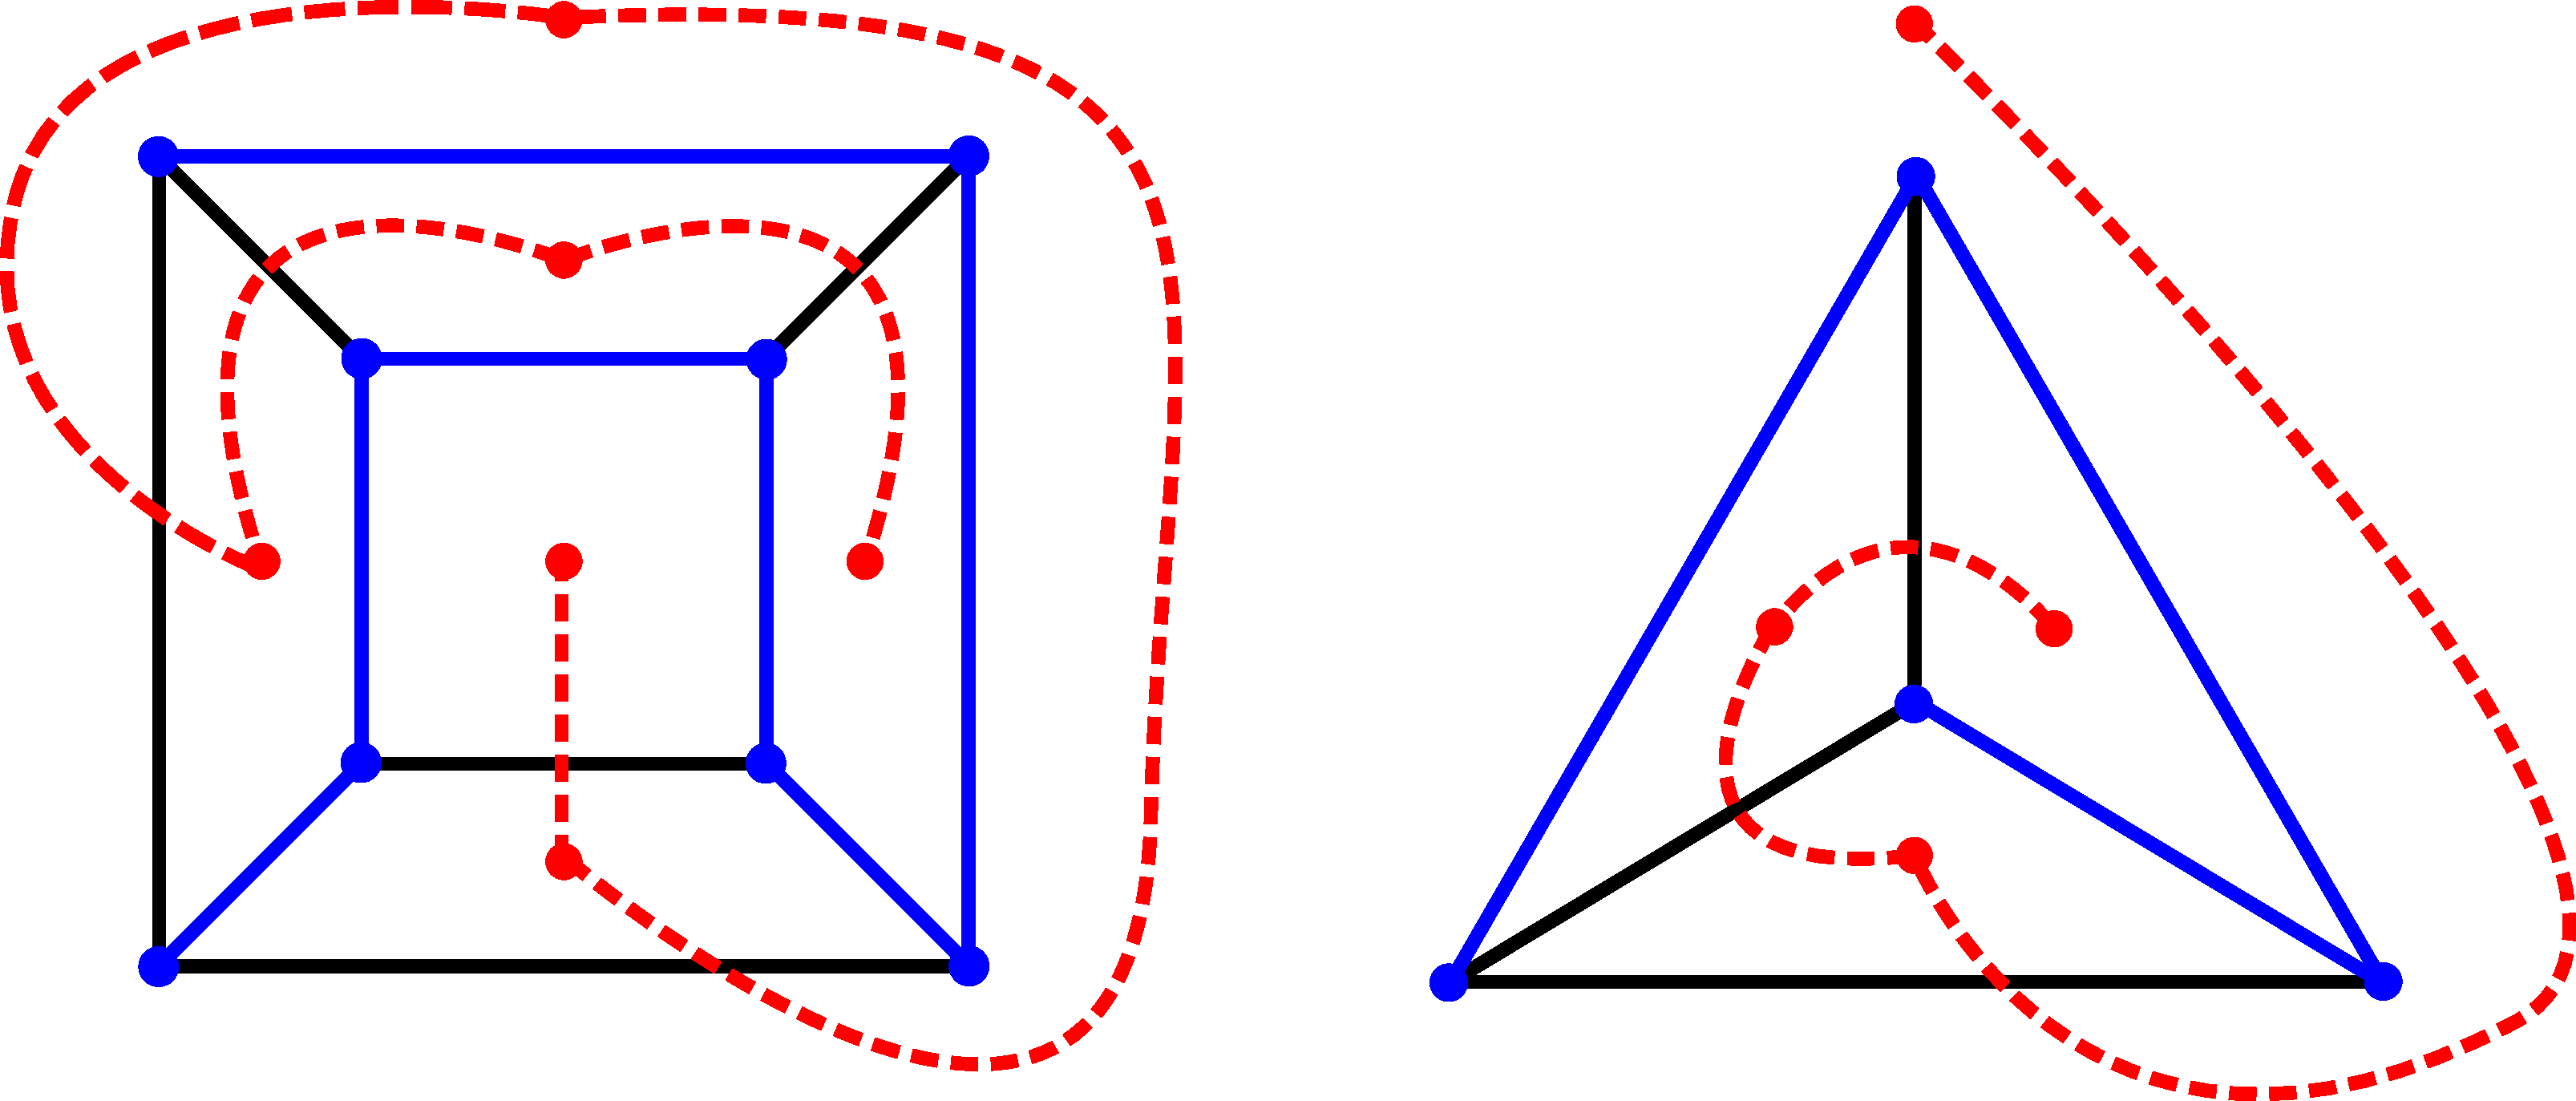
\includegraphics[width=0.7\linewidth]{./grafiken/duale_graphen}
\caption{Veranschaulichung der von Staudtschen Beweisidee}
\label{fig:duale_graphen}
\end{figure}

Der planare Graph des Hexaeders besteht aus einem Quadrat, in das ein kleineres Quadrat symmetrisch einbeschrieben wurde. Die Eckpunkte beider Polygone liegen so auf den eingezeichneten Diagonalen durch den Mittelpunkt.
Die blauen Punkte symbolisieren die acht Ecken des Polyeders bzw. die Knoten des ersten Baums. Die sieben Zweige des Baums sind ebenfalls blau gekennzeichnet. Der duale Graph besteht aus den sechs rot markierten Knoten und den fünf  nicht-durchgezogenen, ebenfalls roten Linien. Der sechste rote Knoten, der anschaulich mit dem Mittelpunkt bzw. einem weiteren roten Knoten zusammenfällt, wurde aus Gründen der Übersichtlichkeit außerhalb des planaren Graphen abgetragen.\\
Der planare Graph zum Tetraeder hat die äußere Form eines gleichseitigen Dreiecks. Die Dreiecksfläche wird punktsymmetrisch vom Mittelpunkt aus mit drei Strecken in drei kongruente Segmente unterteilt. Analog zur Darstellung am Hexaeder sind die Bestandteile des ersten Baums blau hervorgehoben, die des zweiten Graphen rot. Ebenso wurde der vierte Knoten zur Verdeutlichung außerhalb des gleichseitigen Dreiecks abgetragen. \\
\begin{bem} 
Der Eulersche Polyedersatz ist nur für konvexe Polyeder gültig. Man kann sich dessen leicht mit einem Gegenbeispiel für ein nicht-konvexes Polyeder überzeugen.
\end{bem}

Nach dieser Vorbereitung wollen wir nun den zweiten, oben angekündigten Beweis dafür führen, dass es nicht mehr als die fünf uns bekannten regulären Polyeder geben kann: 
\begin{proof}
Wir betrachten ein reguläres Polyeder mit $\mathcal{N}_2$ Flächen. Jede dieser Flächen ist ein reguläres n-seitiges Polygon. 
An jeder der $\mathcal{N}_0$ Ecken treffen k Kanten zusammen.
Jede der $\mathcal{N}_1$ Kanten gehört zu zwei Flächen. Wenn wir die Kanten nach den Flächen abzählen, ergibt sich:  
\begin{align}
\setcounter{equation}{0}
n\mathcal{N}_2= 2\mathcal{N}_1 \label{start1}
\end{align}
Außerdem gehört jede Kante auch zu zwei Ecken. Analog formulieren wir daher: 
\begin{align}
k\mathcal{N}_0=2\mathcal{N}_1 \label{start2}
\end{align}
Der Eulersche Polyedersatz führt beide Gleichungen in einer Formel zusammen: 
\begin{align}
\frac{2\mathcal{N}_1)}{k} + \frac{2\mathcal{N}_1}{n} - \mathcal{N}_1 &= 2 \\
\Leftrightarrow \frac{1}{k} + \frac{1}{n} - \frac{1}{2} &= \frac{1}{\mathcal{N}_1}\\
\Leftrightarrow \frac{1}{k} + \frac{1}{n}  &= \frac{1}{\mathcal{N}_1} + \frac{1}{2}\label{zusammenfassung}
\end{align}
\end{proof}
Wir wissen einerseits, dass ein Polygon mindestens drei Seiten hat und, dass an jeder Ecke wenigstens drei Flächen zusammentreffen, d.h. es gilt $n\geq 3$ und $k\geq 3$. Andererseits ist die Anzahl Kanten $\mathcal{N}_1$ des Polyeders eine natürliche Zahl, sodass die rechte Seite in Gleichung ()\ref{zusammenfassung}) größer als $\frac{1}{2}$ ist. Wenn nun auf der linken Seite der Gleichung jedoch $k$ und $n$ größer als 3 wären, könnte die linke Seite insgesamt nicht echt größer als $\frac{1}{2}$  sein. Diese Feststellungen schränken die Zahl der Fälle ein: Wir brauchen nur noch zu untersuchen, welche Werte $k$ bzw. $n$ annimmt, wenn $n=3$ bzw. $k=3$ festgelegt wird.\\
Wir beginnen mit $k=3$.
Gleichung(\ref{zusammenfassung}) kann dann umgeformt werden zu: 
\begin{align}
\frac{1}{n}- \frac{1}{6}= \frac{1}{\mathcal{N}_1} \label{kfix}
\end{align}
Damit die Differenz echt positiv ist, kann $n$ nur die Werte $3, 4, 5$ annehmen. Dass die Differenz größer 0 sein muss ist klar, da $\mathcal{N}_1 \in \mathbb{N}$. 
Wenn wir nacheinander $3,4$ und $5$ einsetzen in (\ref{kfix}), erhalten wir für $\mathcal{N}_1$ die Werte $6, 12$ und $30$.\\
Fixieren wir $n$ statt $k$, erhalten wir analog diese Gleichung: 
\begin{align}
\frac{1}{k}- \frac{1}{6}= \frac{1}{\mathcal{N}_1} \label{nfix}
\end{align}
 Dementsprechend kann $k$ ebenfalls nur $3,4$ oder $5$ sein. Die Anzahl der Kanten beträgt wiederum $6, 12$ oder $30$.\\
Im letzten Schritt setzen wir die Werte für $n,k$ und $\mathcal{N}_1$ in (\ref{start1}) und (\ref{start2}) bzw. in die Gleichungskette $n\mathcal{N}_2=2\mathcal{N}_1=k\mathcal{N}_0$ ein und erhalten die Werte für $\mathcal{N}_0$ und $\mathcal{N}_2$. Die Ergebnisse sind in der untenstehenden Tabelle aufgeführt.
\begin{center}
\begin{tabular}{p{3.5cm}|c|c|c}
$n\mathcal{N}_2=2\mathcal{N}_1=k\mathcal{N}_0$ & Anz. Ecken $\mathcal{N}_0$& Anz. Flächen $\mathcal{N}_2$& Bezeichnung\\ \hline
$3\mathcal{N}_2=2 \cdot 6=3\mathcal{N}_0$& 4 & 4 & Tetraeder\\ \hline
$3\mathcal{N}_2=2 \cdot 12=4\mathcal{N}_0$& 8 & 6 & Hexaeder \\ \hline
$3\mathcal{N}_2=2 \cdot 30=5\mathcal{N}_0$& 12 & 20 & Ikosaeder\\ \hline
$4\mathcal{N}_2=2 \cdot 12=3\mathcal{N}_0$& 6 & 8 & Oktaeder \\ \hline
$5\mathcal{N}_2=2 \cdot 30=3\mathcal{N}_0$& 20 & 12 & Dodekaeder

\end{tabular}
\end{center}
